\documentclass[12pt,a4paper,final]{article}
\usepackage[latin1]{inputenc}
\usepackage[authoryear]{natbib}
\usepackage[T1]{fontenc}
\usepackage{amsmath}
\usepackage{amsfonts}
\usepackage{amssymb}
\usepackage{setspace}
\usepackage[pagewise]{lineno}
\usepackage{graphicx,epstopdf}
\usepackage{subfigure}
\usepackage[verbose,a4paper,tmargin=2.4cm,bmargin=2.4cm,lmargin=2.4cm,rmargin=2.4cm]{geometry}
\usepackage[hidelinks]{hyperref}
\usepackage{url}
\usepackage{setspace}
%\doublespacing

% Use the PLoS provided bibtex style
\bibliographystyle{plos2009}

\usepackage{color,ulem} % package for text color comments

\author{Vasilis Dakos and Leo Lahti}

\title{
\begin{figure}[h]
\begin{left}

\includegraphics[scale=0.55]{logoEWS.eps}
\end{left}
\end{figure}
\\
Early Warning Signals Toolbox: 
\\ A novel approach for Detecting Critical Transitions
}

\begin{document}
\maketitle

\section{In an nutshell} %Overview
Critical transitions have been identified in seemingly disparate systems ranging from ecology and climate to medicine and finance (Scheffer et al. 2001; Scheffer 2009). %Global finance occasionally suffers from market crashes (May et al. 2008), while asthma attacks (Venegas et al. 2005) and epileptic seizures (McSharry et al. 2003) are examples of sudden medical systemic failures. Abrupt shifts in ocean circulation have occurred in the past climate (Rahmstorf 2002) and may be triggered again under present trends of global environmental conditions (Lenton et al. 2008).
Acknowledging the existence of such critical transitions is only the first step for avoiding them. What we are currently lacking are tools that we can use to foresee such upcoming transitions. Being able to quantify the probability of a critical transition happening would be of unperceived value. Unfortunately, for most systems, we neither have enough records of past transitions nor reliable models to study their behavior. Nonetheless, recent work has proposed an alternative, novel way of approaching this challenge. What if, instead of building case-specific models or indicators, we could be able to measure the resilience of a system- and thus its proximity to a critical transition- using a more generic approach? Complex systems theory appears to have provided us with a potential solution: \textit{\textbf{generic early-warning signals}} for critical transitions (Scheffer et al. 2009). 
\\
\\
Here, we present our newly developed \textbf{Early Warning Signal Toolbox} designed for the \textbf{estimation} and \textbf{visualization} of fingerprints of upcoming critical transitions from time series data. Our toolbox is characterized by three unique features. \textit{\textbf{First}}, it is of truly generic nature which means that it can be used for any type of system that may experience a critical transition. \textit{\textbf{Second}}, it is based on highly sophisticated published methods that have been already tested in real world cases. \textit{\textbf{Third}}, it is easy to use and it is developed under an open-access, widely-used, statistical program (R Project for Statistical Computing\footnote{http://www.r-project.org}). In what follows we explain in laymen terms the theory behind the development of our toolbox, we present how the toolbox works by providing an example, and we propose how this toolbox can have broader benefits for the understanding and management of complex systems in the future.  

\section{The Early Warning Signals Toolbox - Theory} 

\subsection{Why should we expect Early Warnings before Critical Transitions?}
A simple way to understand why we should expect early warnings before critical transitions is to think of the behavior of a system as the motion of a ball in a landscape of valleys and hilltops (Fig. 1 a). Balls represent the state of the system. Valleys correspond to the basins of attraction of alternative stable states of the system. The width and the steepness of the basin of attraction determine the capacity of the system to absorb a perturbation without shifting to an alternative state, and reflects the resilience of the state of the system. As conditions bring the system close to a critical transition (Fig. 1b), the basin of attraction of the current state of the system shrinks and so does its resilience: even a tiny perturbation is enough to shift the sphere to the alternative valley. At the same time, the steepness of the basin of attraction becomes lower: this means that the same perturbation that may not tip the system, it will definitely take longer to dissipate due to the phenomenon of \textit{\textbf{critical slowing down}} (Fig. 1 b). \textit{Mathematically}, critical slowing down is connected to the fact that close to the critical transition the dominant eigenvalue of the system at equilibrium vanishes and has been proven to be be universal prior to critical transitions  (Wissel 1984; Strogatz 1994). \textit{Practically}, critical slowing down enables us to probe the dynamics of the system in order to assess its resilience and the risk of an upcoming transition. The long time required by a system to recover from a perturbation can serve as early-warning signal for an approaching tipping point (van Nes & Scheffer 2007) (Fig. 1 a1, b1).

\begin{figure}[h]
\begin{center}
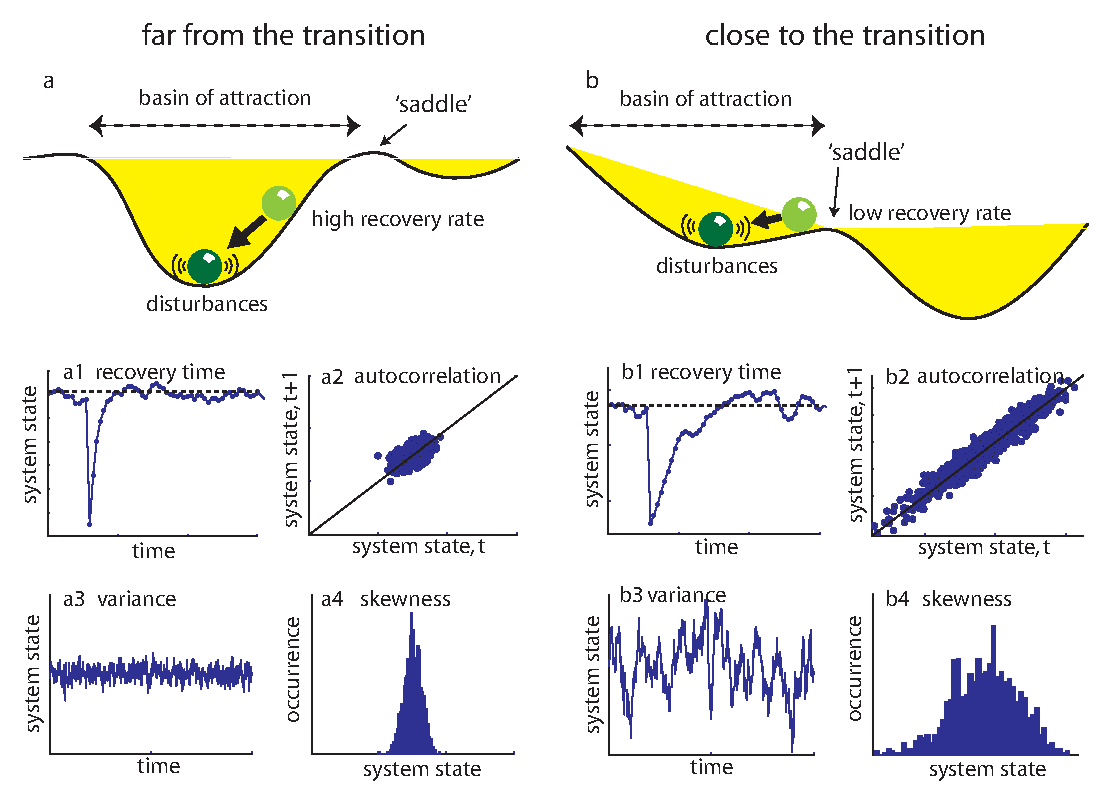
\includegraphics[scale=0.8]{figure1.eps}
\caption{Early-warnings in the dynamics of a system as it approaches a critical transition. Far from the transition resilience is high (a): the system lies in a broad and steep basin of attraction. Small disturbances are damped by high recovery rates back to equilibrium. As a result the time to recover from perturbations is short (a1), the dynamics are characterized by low correlation between subsequent states (a2), low variance (a3), and low skewness (a4). Close to transition resilience is low (b): the system lies in a narrow and flat basin of attraction. Small disturbances are not effectively damped due to critical slowing down. As a result the time to recover from perturbations is short (b1), the dynamics are characterized by high correlation (b2), high variance (b3), and high skewness (b4).}
\end{center}
\label{fig:ews_theory}
\end{figure}

\subsection{What are Early Warning Signals?}
While an increase in recovery time after a disturbance is the most direct indicator of the vicinity to a tipping point, for most natural systems it will be very difficult to measure it systematically. Take for instance the impossibility of conducting a perturbation experiment for measuring the resilience of the thermohaline circulation. The fact, however, that all systems are permanently subjected to natural perturbations allows us to identify an approaching tipping point indirectly. First, slowing down leads to an \textit{\textbf{increase in autocorrelation}} (Ives 1995; Held & Kleinen 2004): the state of the system resembles its previous state when it is close to a tipping point (Fig. 1 a2, b2). The resulting increase in `memory' of the system can be measured in the frequency spectrum of the system by simply looking at lag-1 autocorrelation in the pattern of fluctuations (Held & Kleinen 2004). Second, there is an \textit{\textbf{increase in variance}} (Van Nes & Scheffer 2003; Carpenter & Brock 2006) prior to a tipping point: the state of the system will fluctuate more widely around its equilibrium. As perturbations accumulate and are not damped fast enough due to critical slowing down, the variance in the state of the system increases (Fig. 1 a3, b3). Also, the basin of attraction usually, but not necessarily, becomes asymmetric close to a transition (Scheffer et al. 2009) (Fig. 1 a, b). Such asymmetry causes the state of the system to spend more time in the flatter part of the attraction basin. As a result there is an \textit{\textbf{increase in skewness}} (Guttal & Jayaprakash 2008) in the distribution of the monitored system state before a transition (Fig. 1 a4, b4).

\section{The Early Warning Signals Toolbox - Application}
\subsection{General characteristics}
The Early Warning Signals Toolbox is designed to \textbf{estimate} and \textbf{visualize} a series of \textbf{14 different indicators} that reflect the effects of critical slowing down in the signal properties of a system prior to a critical transition (Table 1). In particular:
\begin{itemize}
\item The toolbox works with time series collected by monitoring the state of a system that we suspect it might undergo a critical transition. It requires no more information to a practitioner other than the time series derived from the system.
\item There is no restriction in the type of data that can be processed. Time series may be temperature data, nutrient concentrations, brain activity, stock marker indices or similar. 
\item The versatility of the toolbox allows to study both real world data as well as simulated time series derived from models that are, for instance, developed to understand climatic transitions, ecological shifts or social collapses.
\end{itemize}


\begin{table}[h]
\centering
\caption{List of methods and indicators estimated by the Early Warning Signals Toolbox}  \\ [1ex]
\begin{tabular}{l l}% c c }
\hline
\hline
%\textbf{Method/ Indicator}\\%	&	Rising memory	&	Rising variability	&	Flickering	\\ [0.5ex]
%\hline
Autocorrelation at-lag-1 &	%&	x	&		&	\\
Autoregressive coefficient of AR(1) model	\\ %&	x	&		& 	\\
Return rate &	%&	x	&		&	\\
Spectral density \\%	&	x	&		&	\\
Spectral ratio &	%&	x	&		&	\\
Spectral exponent\\	%&	x	&		&	\\
Standard deviation &	%&		&	x	&	x	\\
Coefficient of variation\\	%&		&	x	&	x \\
Skewness &	%&		&	x	&	x \\
Kurtosis	\\%&		&	x	&	x \\
Conditional heteroskedasticity	&%&		&	x	&	x	\\
BDS test	\\%&		&	x	&	x	\\
Nonparametric drift-diffusion-jump models	&%&	x	&	x	&	x	\\
Potential analysis	\\ [0.5ex]%&		&		&	x	\\ [1ex]
\hline
\hline
\end{tabular}
\label{methods_table}
\end{table}%

\subsection{An example}
Consider the example of a time series that represents a resource that due to increased harvesting is facing the risk of reaching a point of no return at which resource biomass tips to overexploitation (Fig. 2a). Typically, the managing institution of that resource (be it grazing grounds, or fish stocks) has been monitoring the resource prior to the regime shift (Fig. 2b). Despite the fact that the manager is aware of changes in the driving harvesting pressure and the biomass of the resource is slightly declining, it is difficult to assess the resilience of the system in order to take some action. Imagine now, though, that the manager runs the \textbf{\textit{Early Warning Signal Toolbox}} online on her personal computer to get an idea of whether the resource may be losing resilience and approaching a tipping point. Interestingly, the manager will find out that after removing the slow declining trend in mean biomass (red line in Fig. 2b), the residuals of filtering (Fig. 2c) appear to show a rise in autocorrelation and variance (Fig. 2d). Sensitivity analysis to the parameters of the time series analysis don't change that result: different parameter choices give positive trends in autocorrelation and variance (Fig. 2e). The system indeed seems to be close to tipping, resilience is low. Has there also an alternative attractor already appeared? Potential analysis doesn't show so (Fig. 2f). Still the resource is riding the current stable state. Perhaps there is a chance to control the driver and avoid the further undermining of the resilience of the system. 
\\
\\
This is only part of what our toolbox can perform called the \textbf{Quick Detection Analysis (QDA)}. Here we focus only on it as it estimates the flagship indicators for the detection of critical transitions, but we refer to the full capacity of our toolbox below [\ref{sec:resources}].
\\
\\ 
\textbf{QDA} performs three operations:
\begin{enumerate}
\item An \textbf{Indicator trends analysis} of autocorrelation and variance in rolling windows along a time series that can be pre-treated in multiple ways. The practitioner can select to log-transform or interpolate data (if there are missing values or the data are unevenly spaced) (Fig. 2, Box 1), as well as filter the data using smooth, linear, or first-difference detrending from a drop-down menu (Fig. 2, Box 2). In addition, it is possible to choose the size of the rolling window as a percentage of the total time series length with the help of a scroll bar (i.e. choosing a value of 50 the early warnings are estimated with rolling windows half the size of the time series, Fig. 2 upper panel, Box 3).
\item A  \textbf{Trend sensitivity analysis} of autocorrelation and variance. Two scroll bars allow the user to choose the steps for incrementally changing the size of the rolling window and the bandwidth for the smoothing in order to (Fig. 2 middle panel, Box 4, 5). 
\item A \textbf{Potential analysis} to identify alternative attractors by reconstructing a potential landscape from the data. The cutoff level for the estimation of the attractors can be chosen from 0.01 to 0.5 - a low cutoff level makes the method sensitive and increases the chance of recognizing alternative attractors (Fig. 2 lower panel, Box 6).
\end{enumerate}
\\
\\
Simulated data make a nice illustration, but what about real world examples? Go to the application, choose \textit{real climate data} from the drop-down menu and try it yourself!
\\
\\
\textcolor{blue}{here I am imagining fig 2 to be a product of RShiny (should we also add a short video that only goes with the example?)}

\begin{figure}[h]
\begin{center}
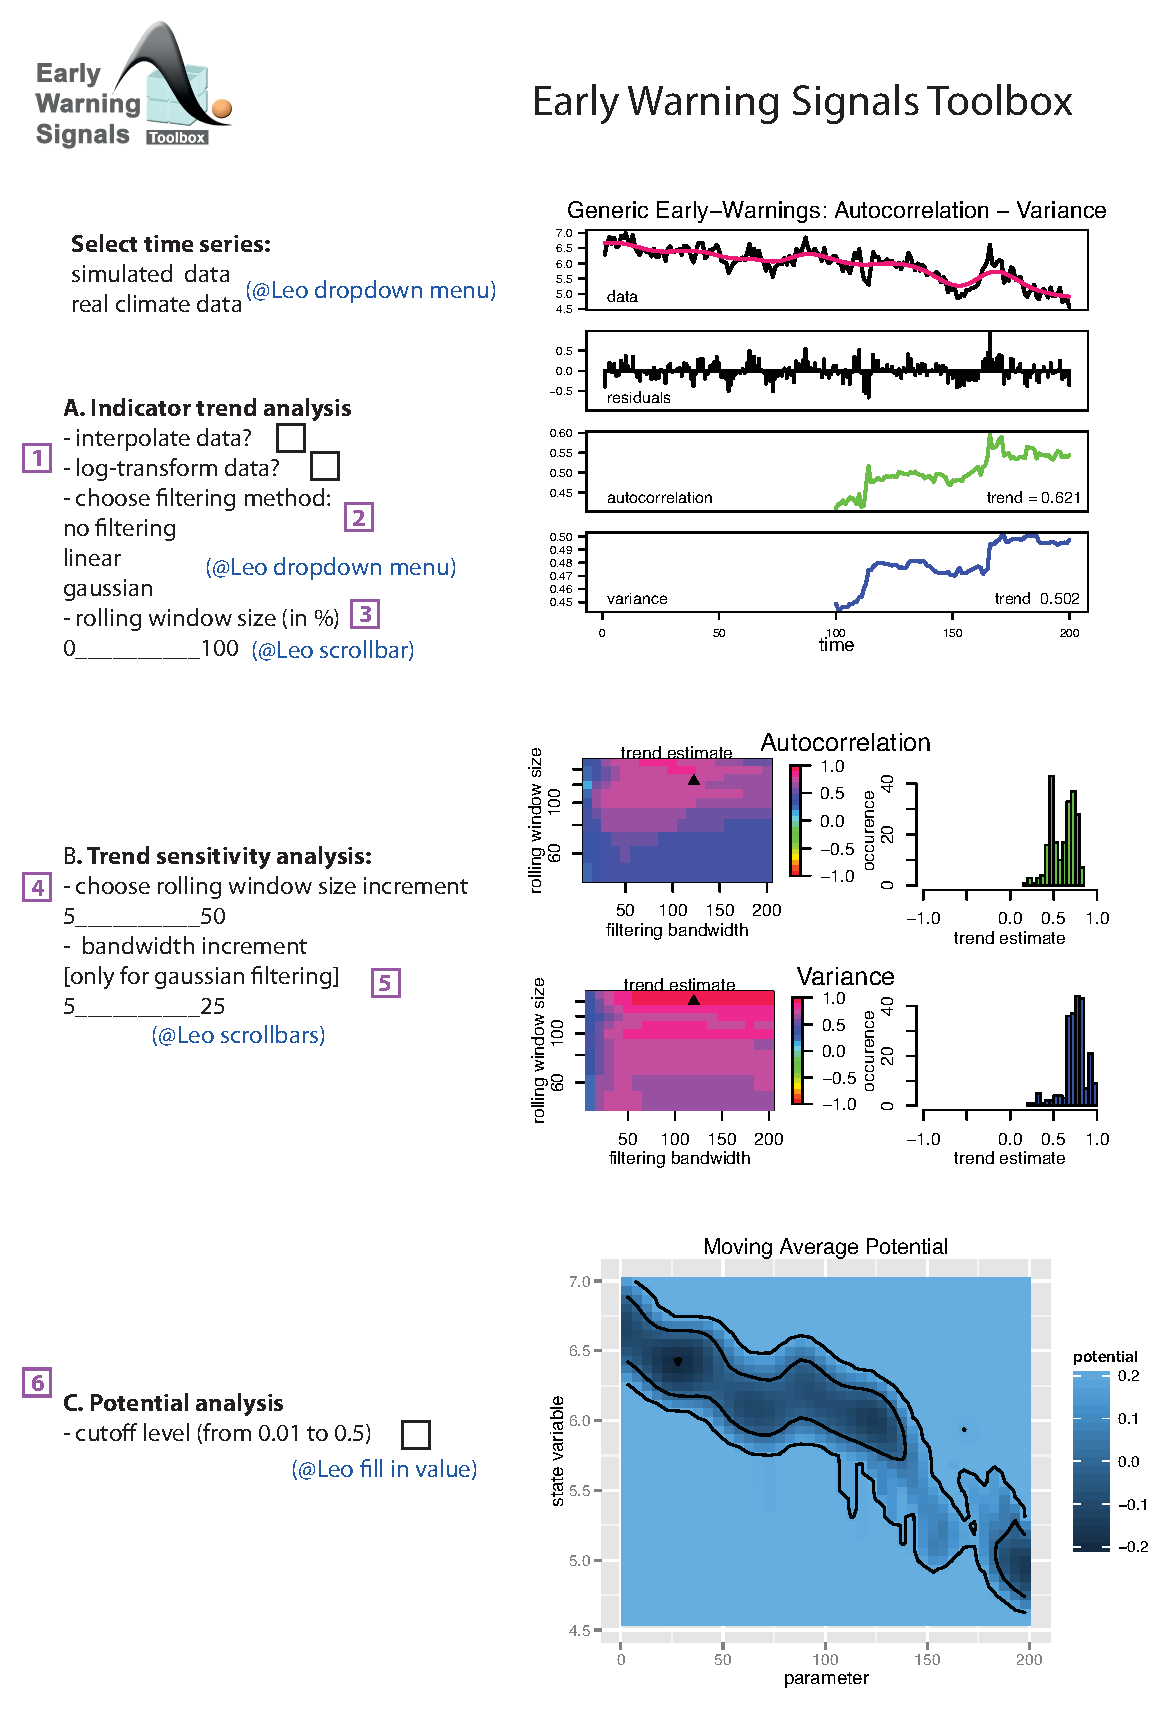
\includegraphics[scale=0.8]{scheme_RShiny_v3.eps}
\caption{Demo Quick Detection Analysis in RShiny}
\end{center}
\label{fig:demoQDA}
\end{figure}

\subsection{Resources} 
\label{sec:resources}
Apart from the toolbox per se, we have developed a complete set of resources available to any practitioner interested in understanding the methodology, using the application, but also contributing to it. In particular, we have a dedicated  \textbf{webpage}\footnote{\url{http://www.early-warning-signals.org}} that hosts all background theoretical and practical information, contains original publications, demonstrates case studies of applying the methods, and provides updates to the science and the community around the theme of early warnings and critical transitions. The toolbox is developed in \textit{R}, the most widely used statistical language and hosted in \textbf{CRAN repository}\footnote{\url{http://cran.r-project.org/web/packages/earlywarnings/index.html}}, which means that it is available to download on any operating system and distributed freely. Lastly, we have hosted the development part of our toolbox on \textbf{github}\footnote{\url{https://github.com/earlywarningtoolbox}}: an open-access, free-sharing platform that allows any interested party to contribute to its further development.

%\href{http://www.early-warning-signals.org}{webpage}
%\href{http://cran.r-project.org/web/packages/earlywarnings/index.html}{CRAN repository}, 
%\href{https://github.com/earlywarningtoolbox}{github}

\section{Potential impact and future perspectives}
One of the most distinct features of our proposed toolbox is its dynamic character and complimentary functionality.

1. it can be used for online as well as after 
2. it can be part of any other tool
3. can work with simulated data and real data.
4. can be further developed- keeping up pace with on going research. This is reflected by our choice to develop this tool in the R statistical computing environment and to make it available on open source project development platforms like github. is related to the fact that we 
\textcolor{blue}{(@Leo: some on open source computing and R?)}


\end{document}

